%
%  jan 28 2012 jh: changes version and date
%
\pdfbookmark[1]{SEISAN Manual}{page1} 
\begin{titlepage}
%\pdfbookmark[1]{First page}{page1} 
\begin{center}
{\huge \bf{SEISAN}}\\[.5cm]
{\huge \bf{EARTHQUAKE ANALYSIS SOFTWARE}} \\[.5cm]
{\large FOR WINDOWS, SOLARIS, LINUX and MACOSX} \\[.5cm]
{\small Version 9.1}\\
%{\small Version 8.3 {\color{red}(9.0)} }\\
%{\small Version 8.2.1 Draft}\\

\begin{figure}[h]
\centering
% \htmlimage{scale=2.0}
% \htmlimage{scale=1.5}
% 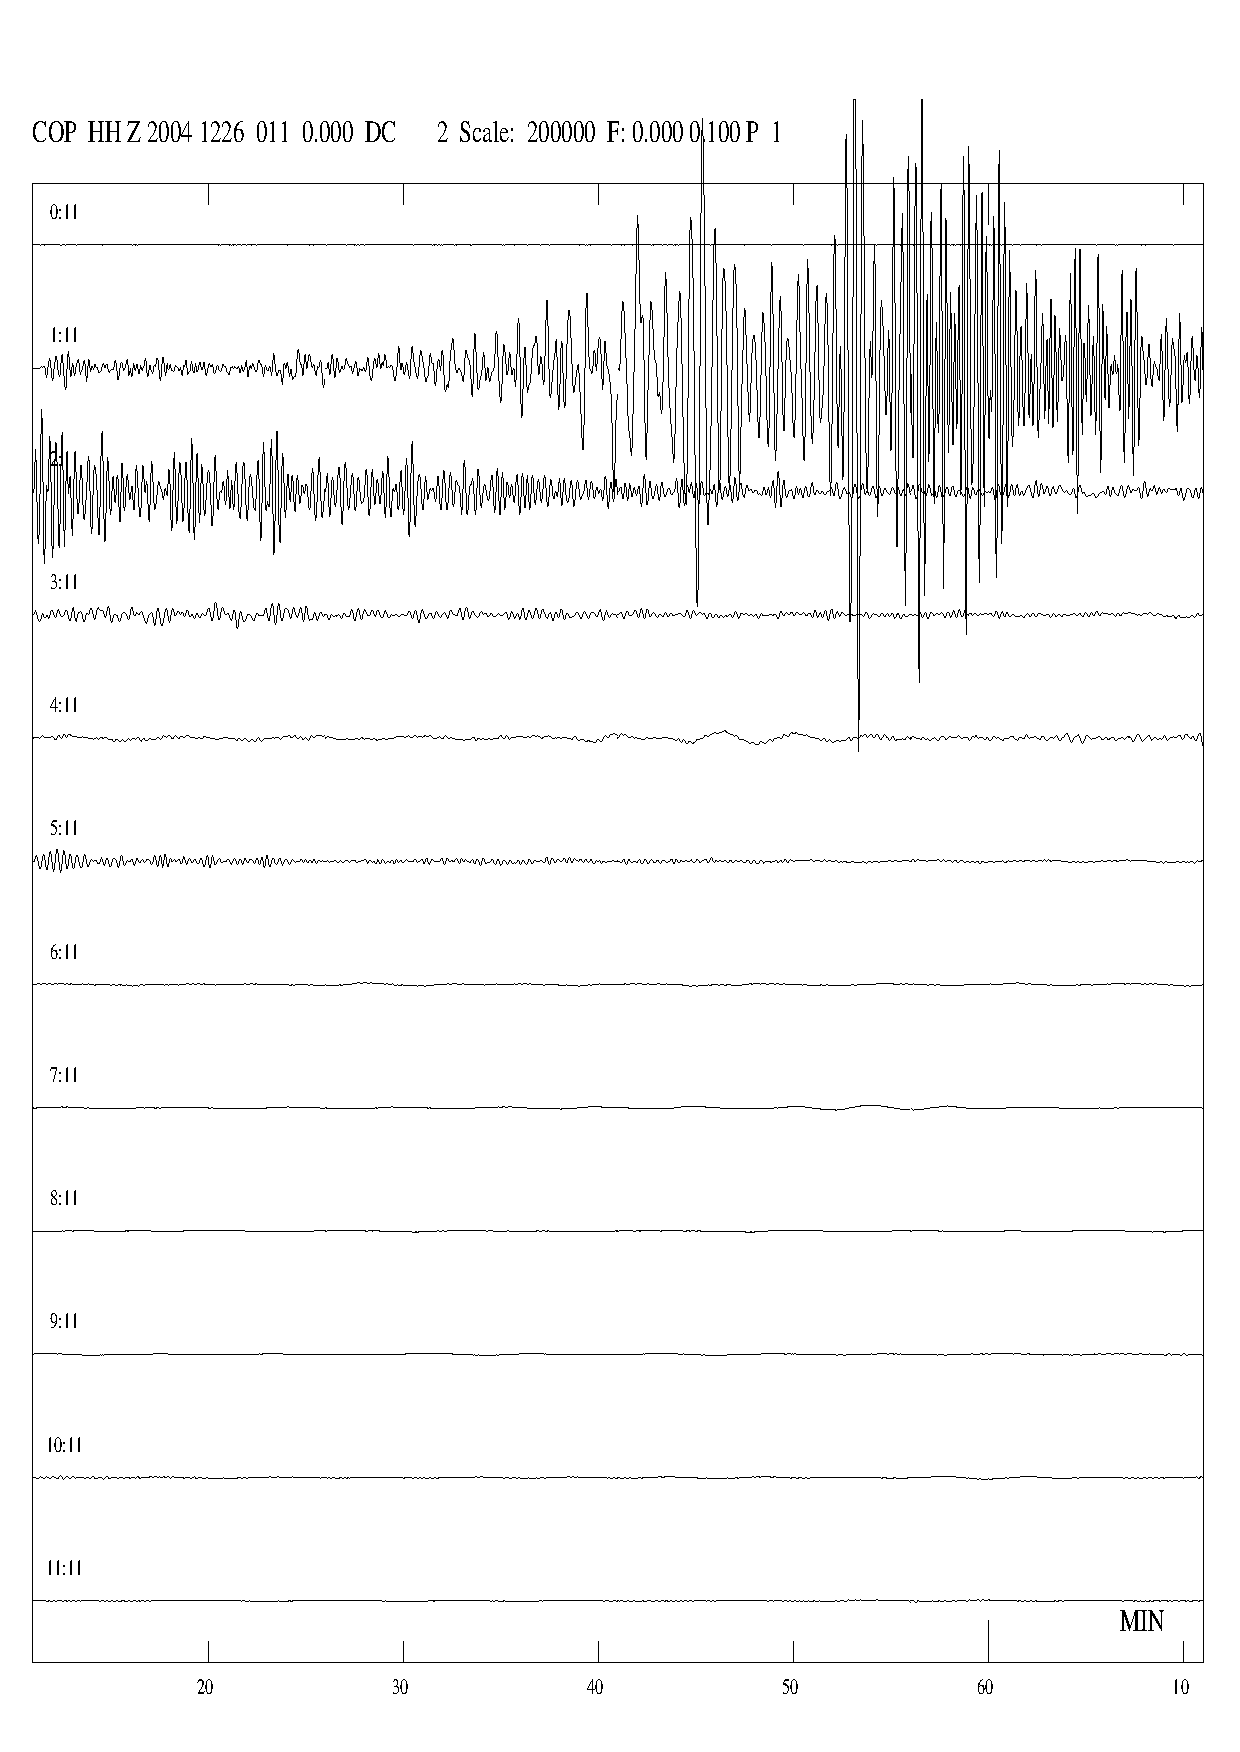
\includegraphics[width=8cm]{fig/cop}\\
% 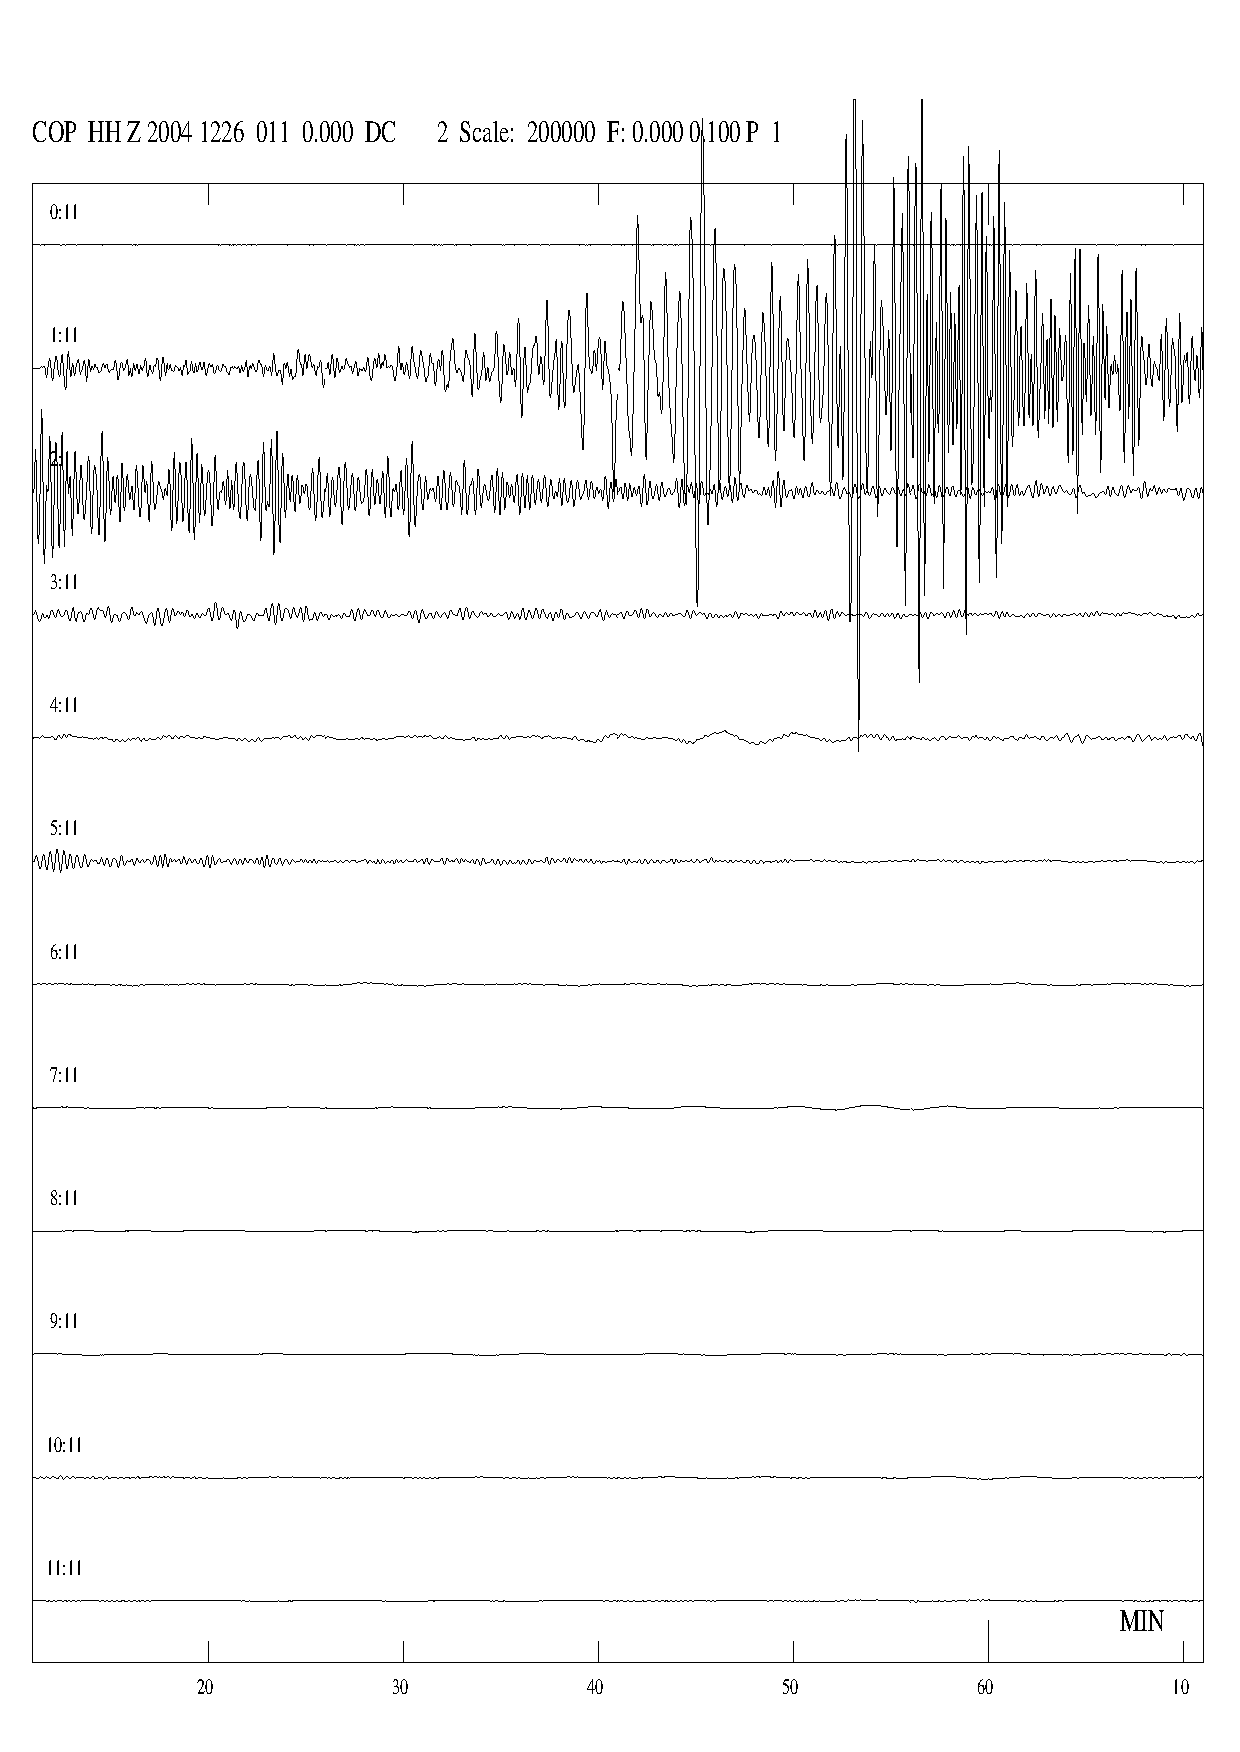
\includegraphics[width=6cm]{fig/cop}\\
% \htmlimage{scale=2.0}
% 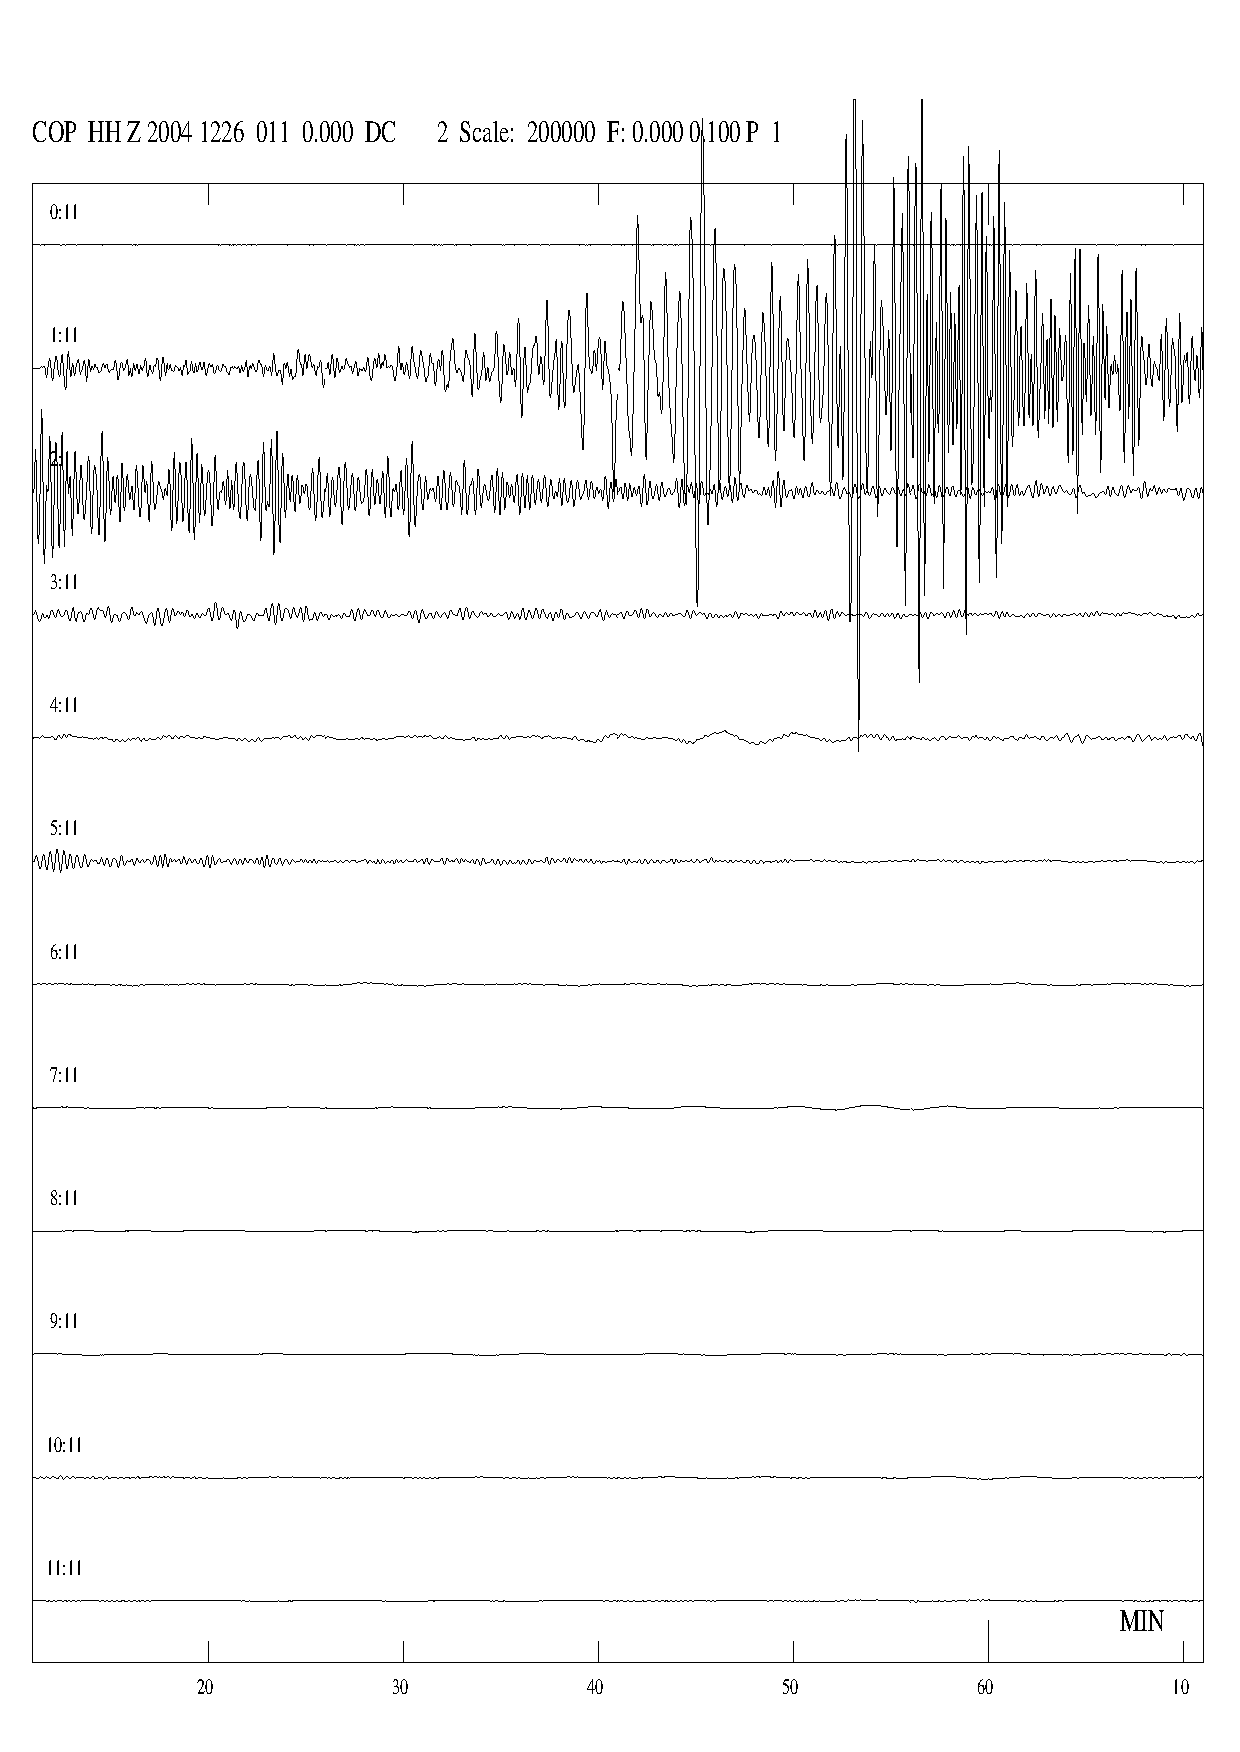
\includegraphics[width=8cm]{fig/cop}\\
\htmlimage{scale=1.0}
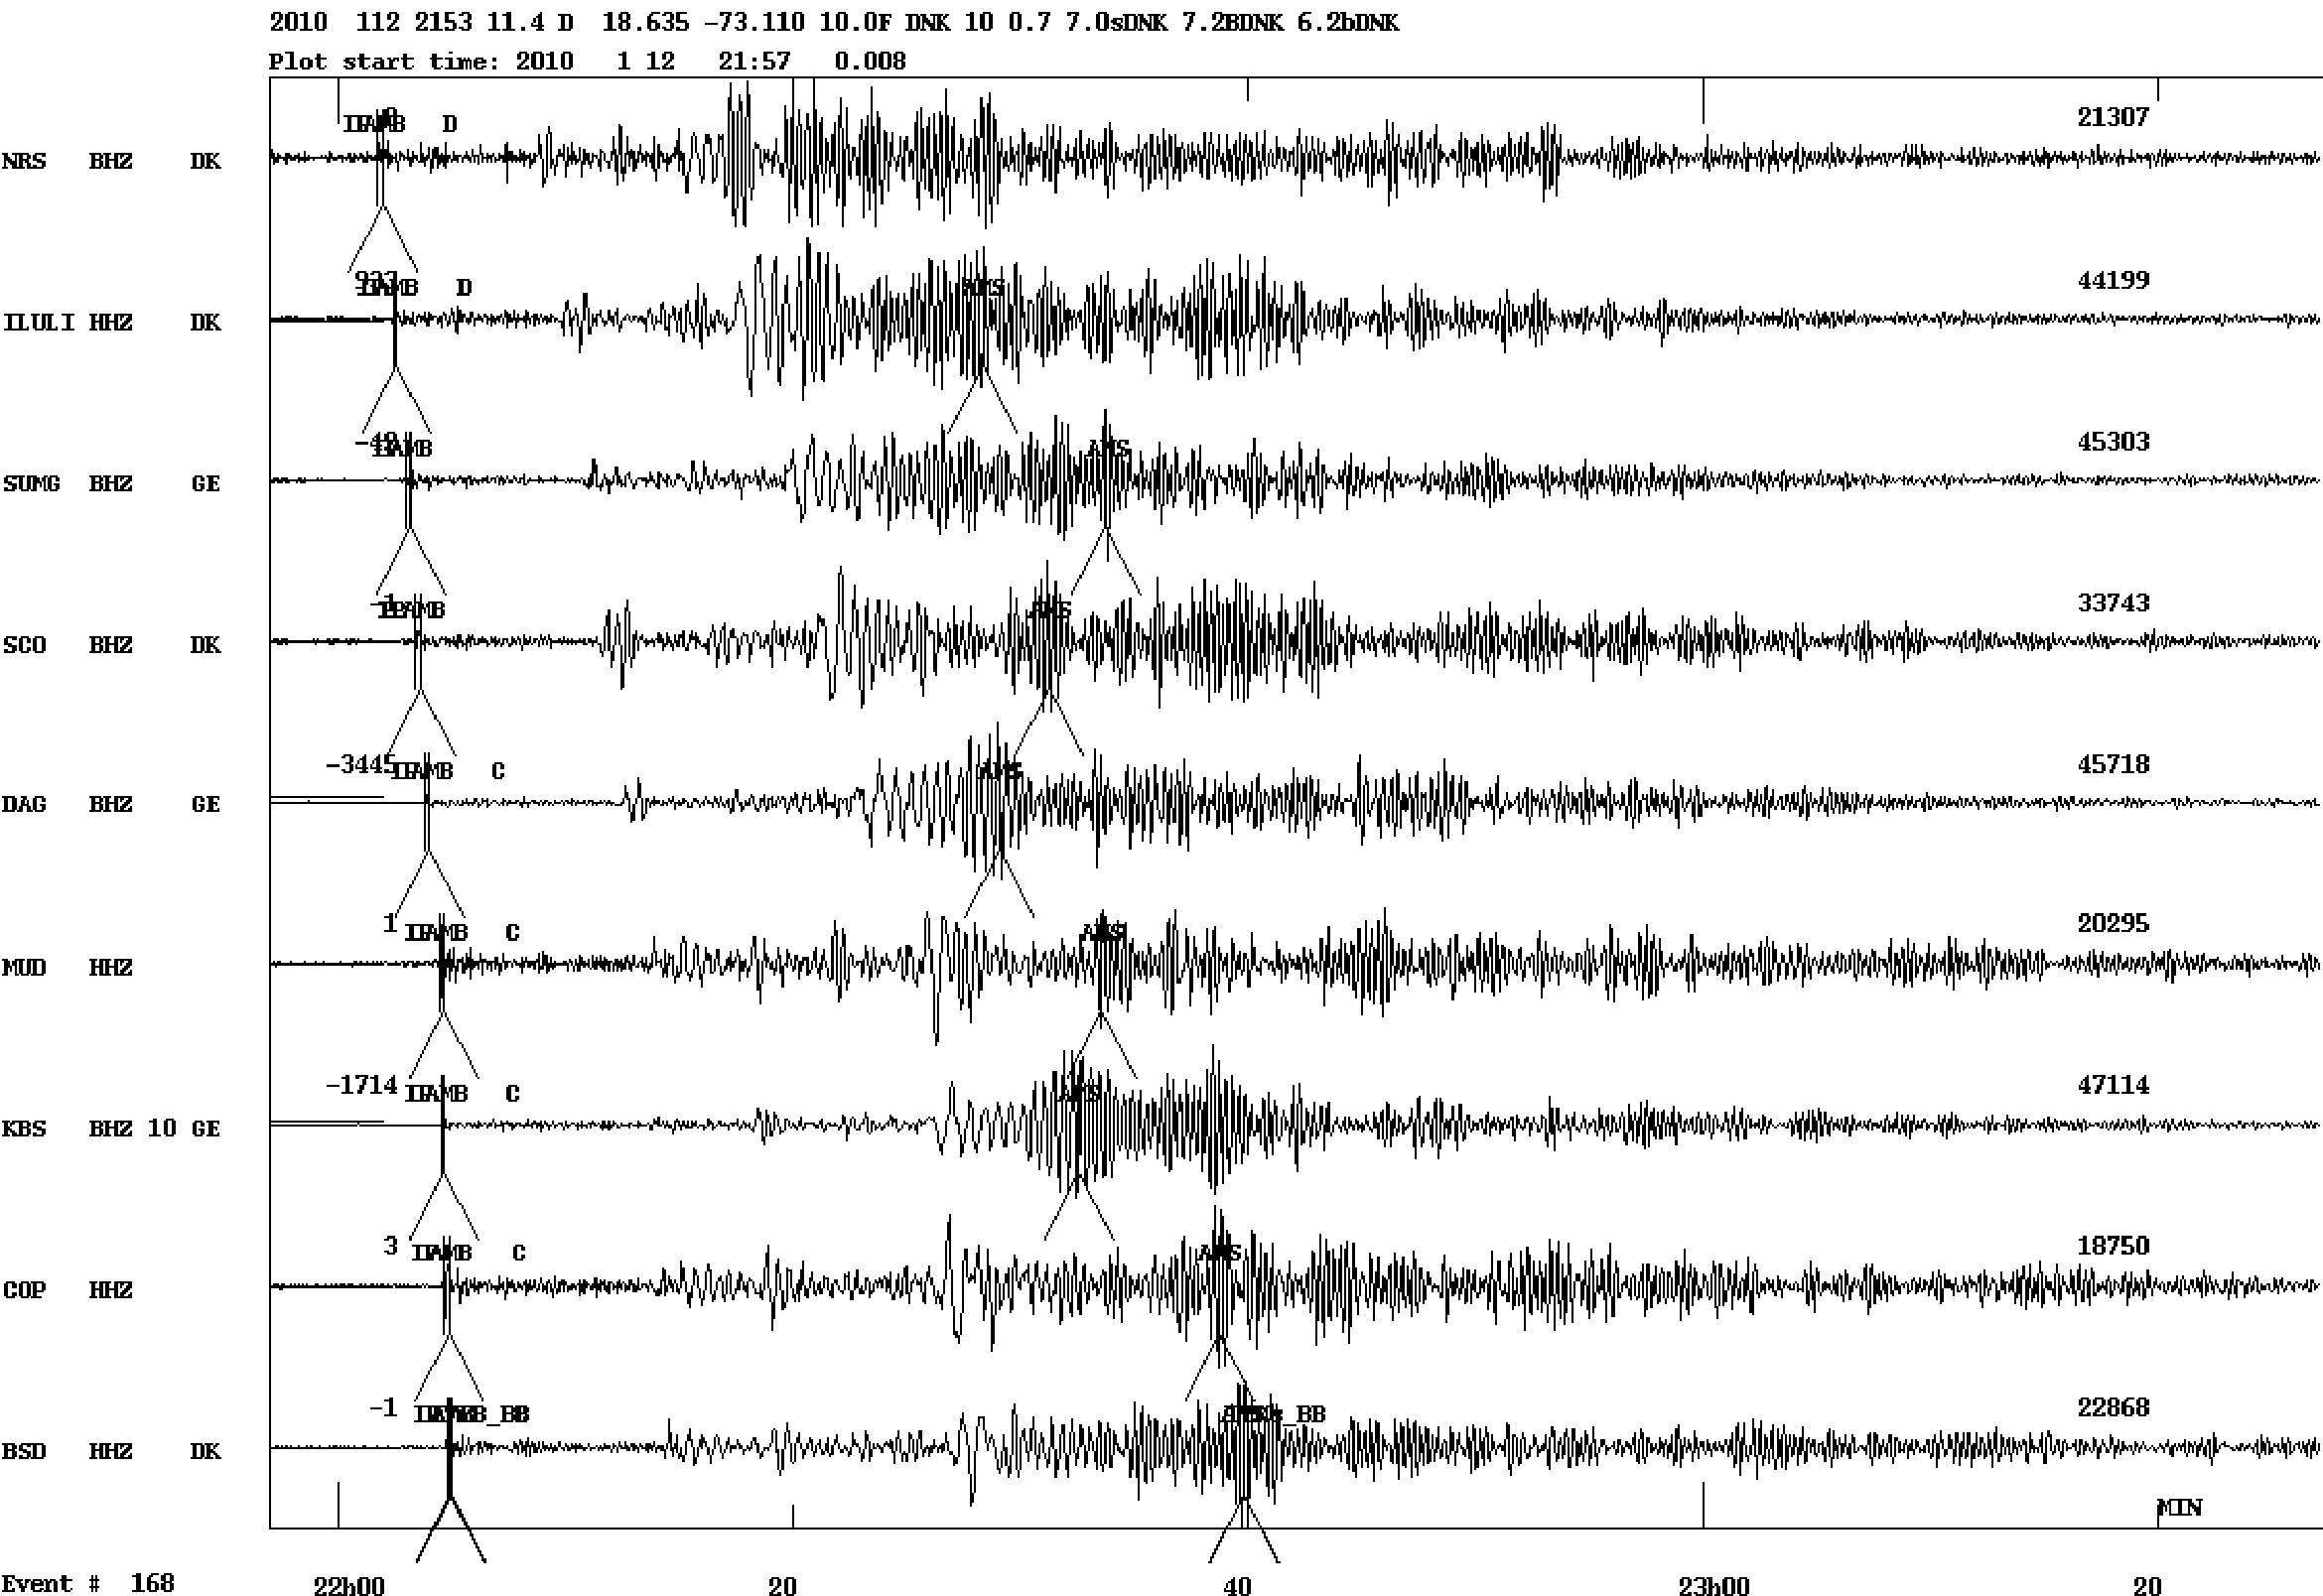
\includegraphics[width=16cm]{fig/haiti2010}\\
\end{figure}

Editors


\begin{tabular}{c}
Lars Ottem\"oller$^{(1)}$ lars.ottemoller@geo.uib.no \\
Peter Voss$^{(2)}$ pv@geus.dk \\
Jens Havskov$^{(1)}$ jens.havskov@geo.uib.no \\
\end{tabular}

\vfill
\vfill
\vfill

\begin{tabular}{cc}
(1) Department of Earth Science & (2) Geological Survey of Denmark and Greenland \\
University of Bergen & \O ster Voldgade 10 \\
Allgaten 41 & 1350 Copenhagen K \\
5007 Bergen & Denmark \\
Norway &  \\
\end{tabular}

\vfill
\vfill
\vfill
\vfill
\vfill
\vfill
\vfill
\vfill
\textbf{November 2012}
\end{center}
%\pdfbookmark[1]{First page}{page1} 
%% \pdfbookmark[n]{Bookmarktitle}{internal_label} 
\end{titlepage}

